\documentclass[a4paper,10pt]{article}
\usepackage[utf8]{inputenc}
\usepackage{polski}
\usepackage{graphicx}
\usepackage{listings}
\usepackage[usenames,dvipsnames]{color}
\addtolength{\hoffset}{-1cm}
\addtolength{\voffset}{-2cm}
\addtolength{\textwidth}{2cm}
\addtolength{\textheight}{3cm}
\usepackage{setspace}
\usepackage{indentfirst}
\usepackage{graphicx}
\lstset{
    language=Matlab,
    basicstyle=\scriptsize,
    aboveskip={1.5\baselineskip},
    columns=fixed,
    showstringspaces=false,
    extendedchars=true,
    breaklines=true,
    tabsize=4,
    prebreak = \raisebox{0ex}[0ex][0ex]{\ensuremath{\hookleftarrow}},
    frame=single,
    showtabs=false,
    showspaces=false,
    showstringspaces=false,
    identifierstyle=\ttfamily,
    keywordstyle=\color[rgb]{0,0,1},
    commentstyle=\color[rgb]{0.133,0.545,0.133},
    stringstyle=\color[rgb]{0.627,0.126,0.941},
    numbers=left,
    numberstyle=\tiny,
    stepnumber=1,
    numbersep=5pt,
    captionpos=b,
    escapeinside={\%*}{*)}
}

\def\figurename{Rys.}
\def\lstlistingname{Fun.}

\title{Informatyczne Systemy Sterowania \\ \large Ćwiczenie 4: Sterowanie ekstremalne}

\author{Adam Jordanek 168139, Tomasz Klimek 168092}

\begin{document}
\maketitle

\section{Wstęp}\label{sec:wstęp}
\subsection{Cel ćwiczenia}
%TODO!!!!! SKOPIOWANE Z LISTY
Celem  ćwiczenia jest symulacja działania systemu sterowania ekstremalnego. Sterowaniem 
ekstremalnym nazywamy zadanie sterowania polegające na doprowadzeniu poprzez odpowiednią
zmianę wielkości sterujących do ekstremalnej wartości wielkości sterowanej (lub ekstremalnych 
wartości wielkości sterowanych w przypadku obiektu wielowyjściowego)

\subsection{Plan badań} 
\begin{enumerate}
	\item Symulacja systemu sterowania ekstremalnego - Algorytm 1
	
	\item Symulacja systemu sterowania ekstremalnego - Algorytm 2
	
	\item Symulacja systemu sterowania ekstremalnego - Algorytm 3
	
\end{enumerate}

\subsection{Podział zadań. } 
\begin{enumerate}
		\item Jordanek Adam - 
		\item Klimek Tomasz -
\end{enumerate}

\newpage
\section{Realizacja planu i wyniki}
W zadaniu sterować będziemy dwa obiekty przedstawione przy pomocy poniższych równań.
\begin{eqnarray}
	y = F(u, a, b, c) = (u^{(1)} - a)^2 + (u^{(2)} - b)^2 + c\\
	y = F(u, a, b, c, A, B, \omega_1, \omega_2, t) = (u^{(1)} - (a + Asin(\omega_1t)))^2 + (u^{(2)} - (b + Bsin(\omega_2t)))^2 + c
\end{eqnarray}
Podczas ćwiczenia przyjęliśmy następujące wartości parametrów. \\
$a=1, b=2, c=3, A=2, B=4, \omega_1=0.5, \omega_2=0.25$
%--------------------------------------------------------------------------------------------------------------------------------
%ZADANIE 1
%--------------------------------------------------------------------------------------------------------------------------------
\subsection{Symulacja systemu sterowania ekstremalnego – wersja 1. algorytmu.}

\subsubsection{Obiekt (1).}
W pierwszym zadaniu do wyznaczenia ekstremów posłuży nam poniższa funkcja.
\begin{eqnarray}
	u_n^{(i)} = u_{n-1}^{(i)}-kd_n^{(i)}\\
	d_n^{(i)} = {F(u_{n-1}) - F(u_{n-2}) \over u_{n-1}^{(i)} - u_{n-2}^{(i)}}
\end{eqnarray}

Jednak dla ułatwienia ćwiczenia powyższy algorytm zmodyfikujemy do poniższej postaci.
\begin{eqnarray}
	u_n^{(i)} = u_{n-1}^{(i)}-kd_n\\
	d_n = {F([\begin{array}{ll} u_{n-1}^{(1)} + \Delta u & u_{n-1}^{(2)} + \Delta u\end{array}]) - F(u_{n-1}) \over \Delta u}
\end{eqnarray}

Z powyższych równań widać, że wartość $d$ to pochodna przyrostu wartości funkcji $F(u)$.
Następnie testować będziemy wpływ parametru $k$, oraz stanu początkowego wejścia $u_0$ na przebieg sterowania przy użyciu odpowiedniej funkcji.
\begin{lstlisting}[caption=Funkcja testująca algorytm 1 dla obiektu 1.]
function alg1fun1(u, kstart, kstep, kstop)
    color = char('y', 'k', 'b', 'g', 'r', 'm');
    hold all;
    k = kstart;
    c = 1;
    
    while(k <= kstop)
        epsilon = 0.1;
        delta = 0.1
        u1(1) = u(1);
        u2(1) = u(2);
        y(1) = funkcja1([u(1) u(2)]);
        i = 1;
        d(1) = 1;
        
        while(epsilon < abs(d(i)))
            a=(funkcja1([u1(i)+delta u2(i)+delta]) - funkcja1([u1(i) u2(i)]));
            d(i+1) =  a / delta;
            u1(i+1) = u1(i) - k * d(i+1);
            u2(i+1) = u2(i) - k * d(i+1);
            y(i+1)= funkcja1([u1(i) u2(i)]);
            i = i + 1;
        end

        figure(1);
        hold on;
        plot(u1, y, '*b');  plot(u2, y, '*r');
        figure(2);
        hold on;
        plot(d, strcat('-', color(mod(c,6)+1)));
        
        c = c + 1;
        k = k + kstep;
        clear u1; clear u2; clear d; clear y;
    end
end
\end{lstlisting}

\newpage Na początku sprawdzimy jaki wpływ na przebieg sterowania ma stan początkowy wejścia $u_0$, ustawiając $k=0.1$ i symulując sterowanie dla trzech różnych wartości $u_0$.
\begin{figure}[!h]
    \centering
	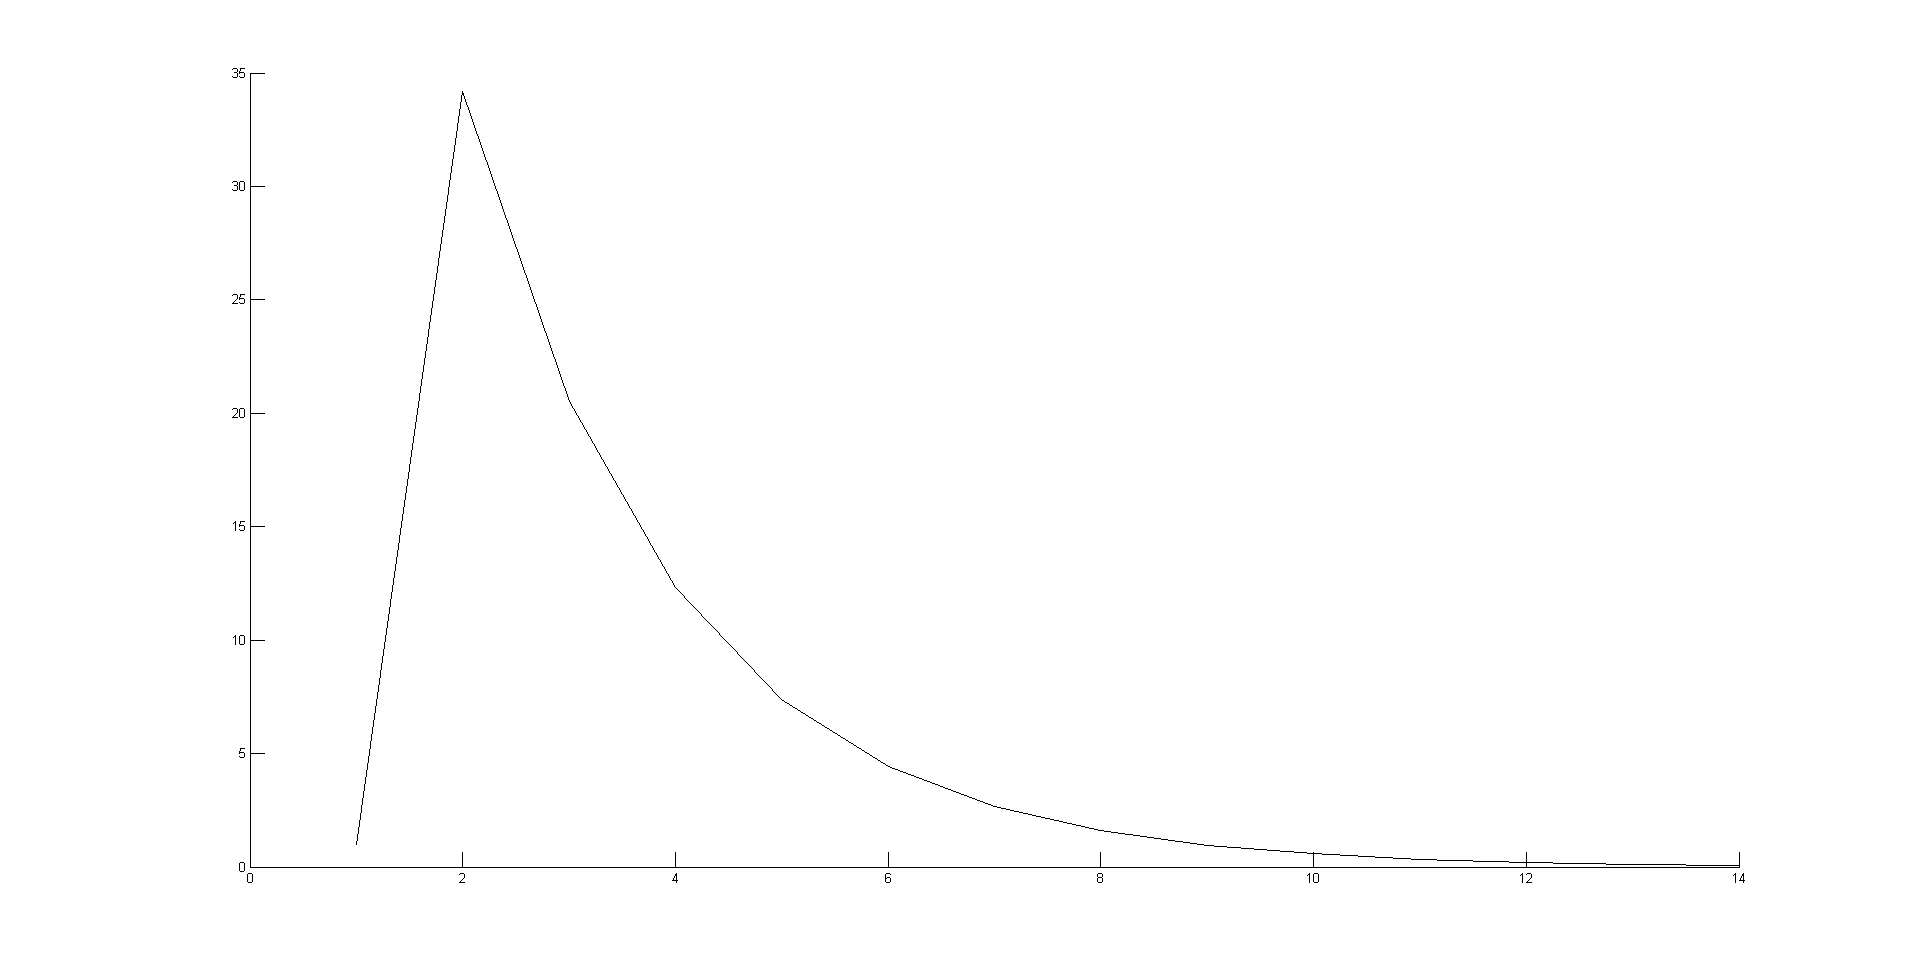
\includegraphics[width=120mm]{CW4-alg1fun1-u10_10-k01-d.png}
	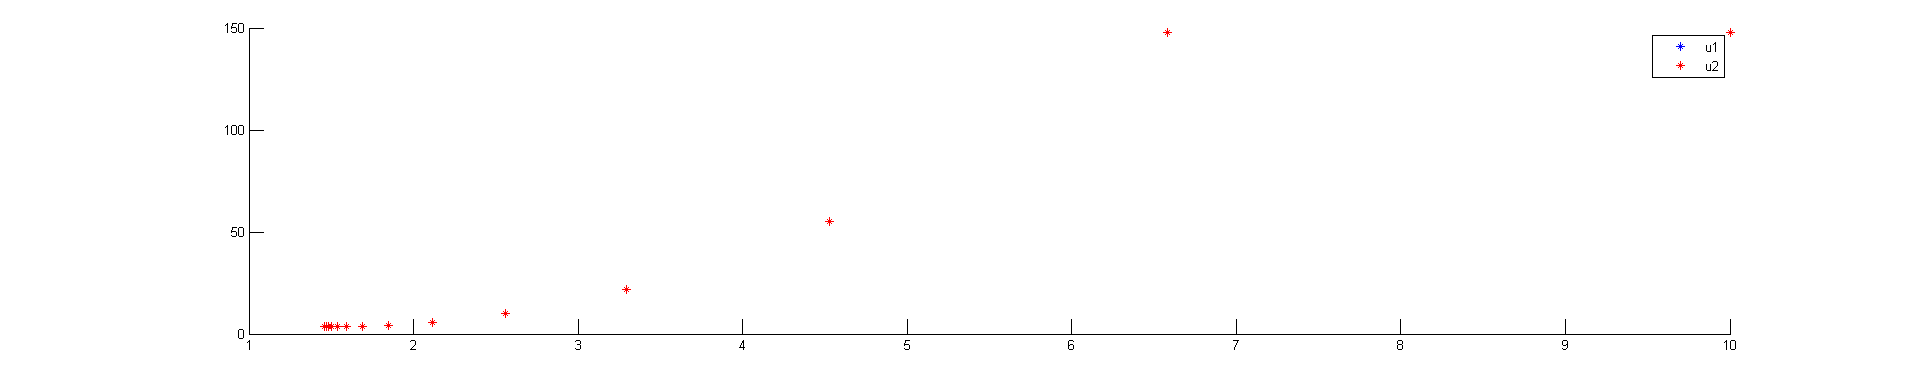
\includegraphics[width=120mm]{CW4-alg1fun1-u10_10-k01-u.png}
	\caption{Wykres wykres wartości $d$, oraz $u^{(1)}$ i $u^{(2)}$ dla $u_0=[10 \quad 10]$.}
    \label{fig:Rysunek}
\end{figure}
\begin{figure}[!h]
    \centering
	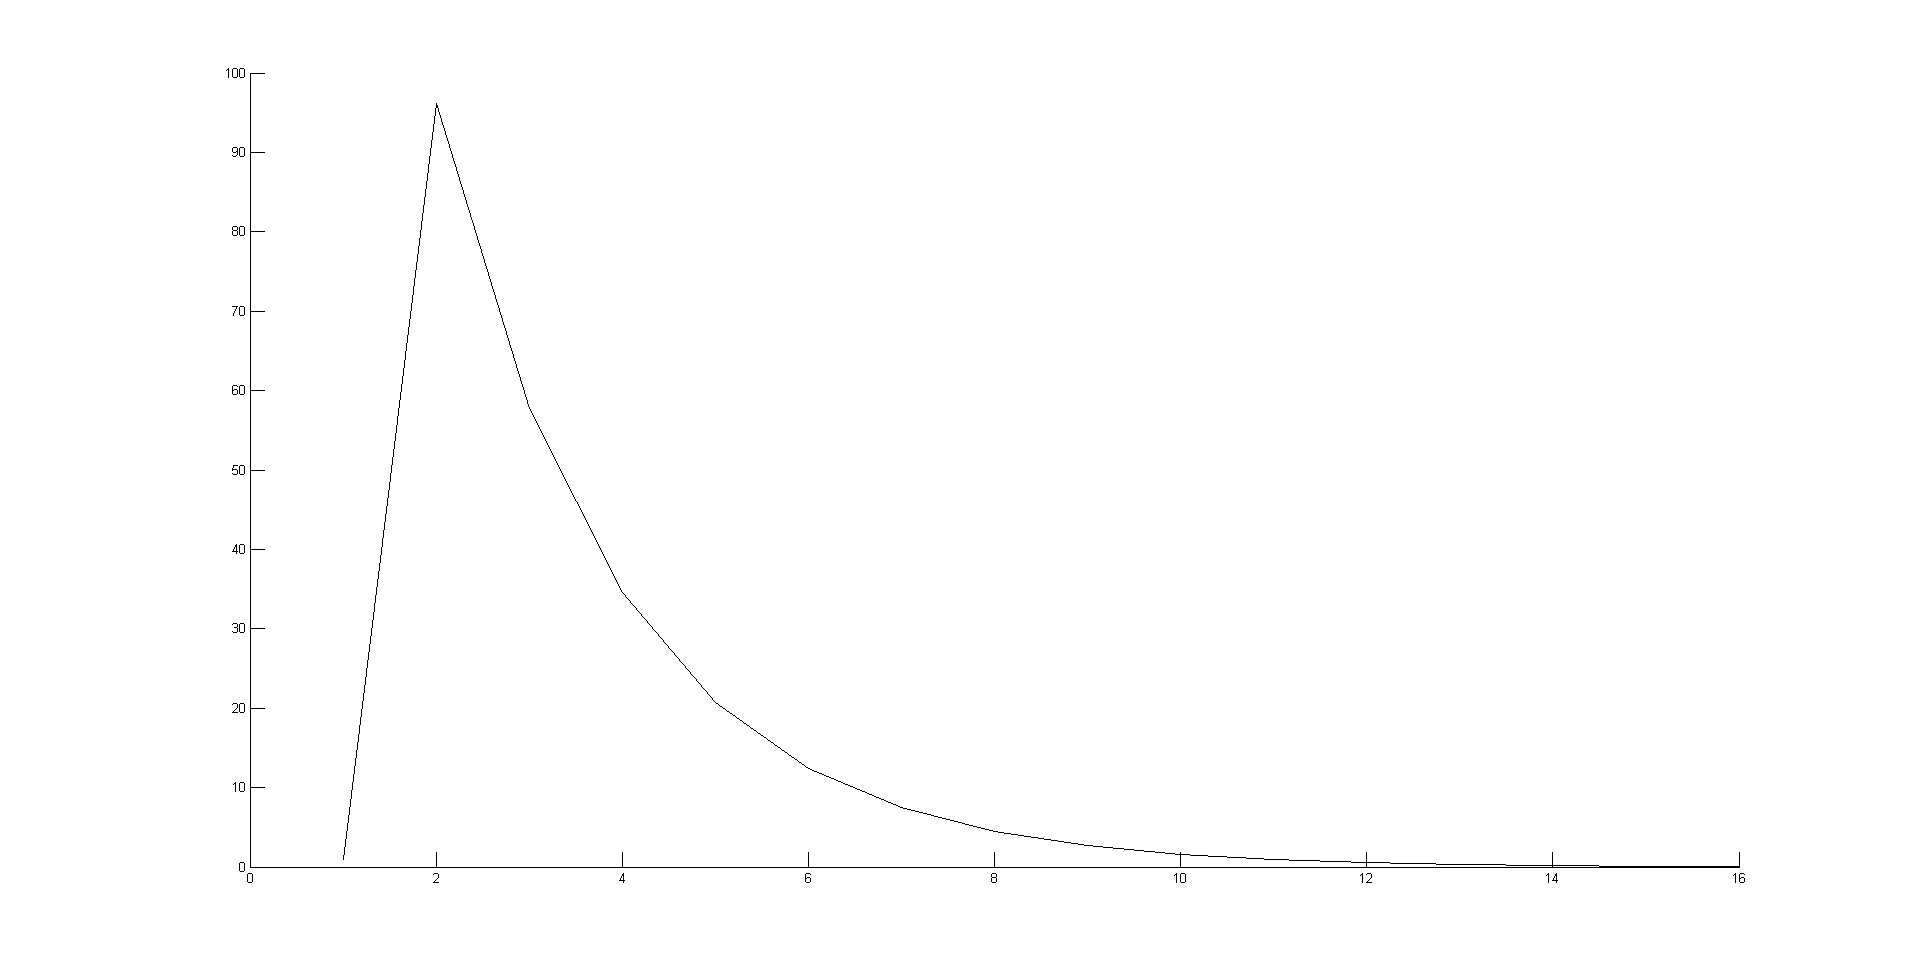
\includegraphics[width=120mm]{CW4-alg1fun1-u10_41-k01-d.png}
	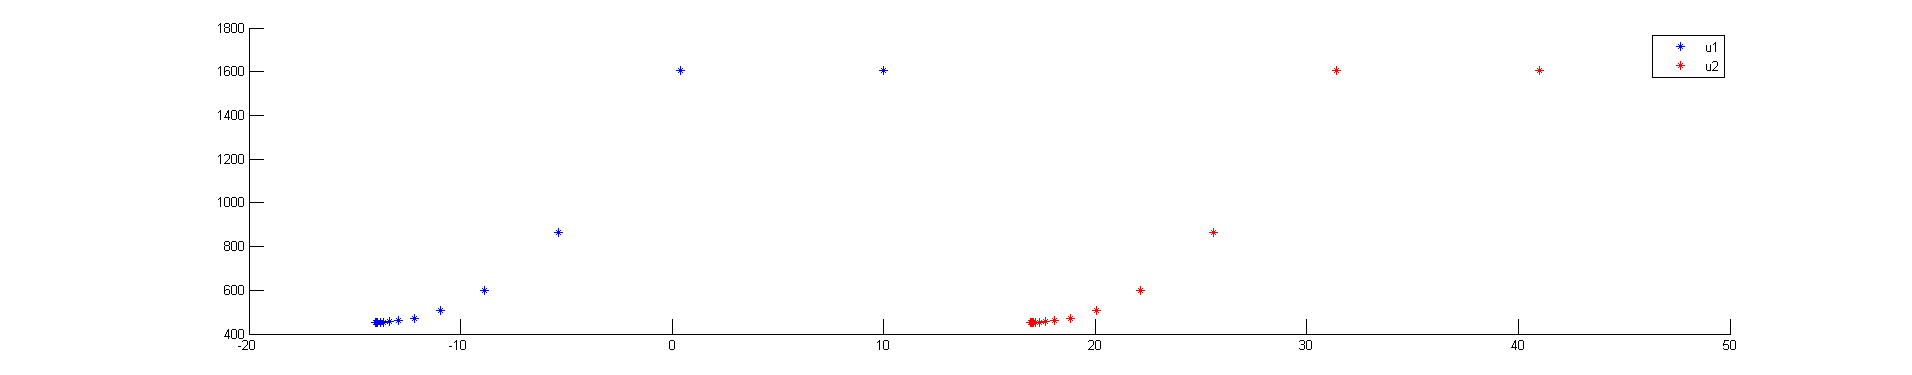
\includegraphics[width=120mm]{CW4-alg1fun1-u10_41-k01-u.png}
	\caption{Wykres wykres wartości $d$, oraz $u^{(1)}$ i $u^{(2)}$ dla $u_0=[10 \quad 41]$.}
    \label{fig:Rysunek}
\end{figure}
\begin{figure}[!h]
    \centering
	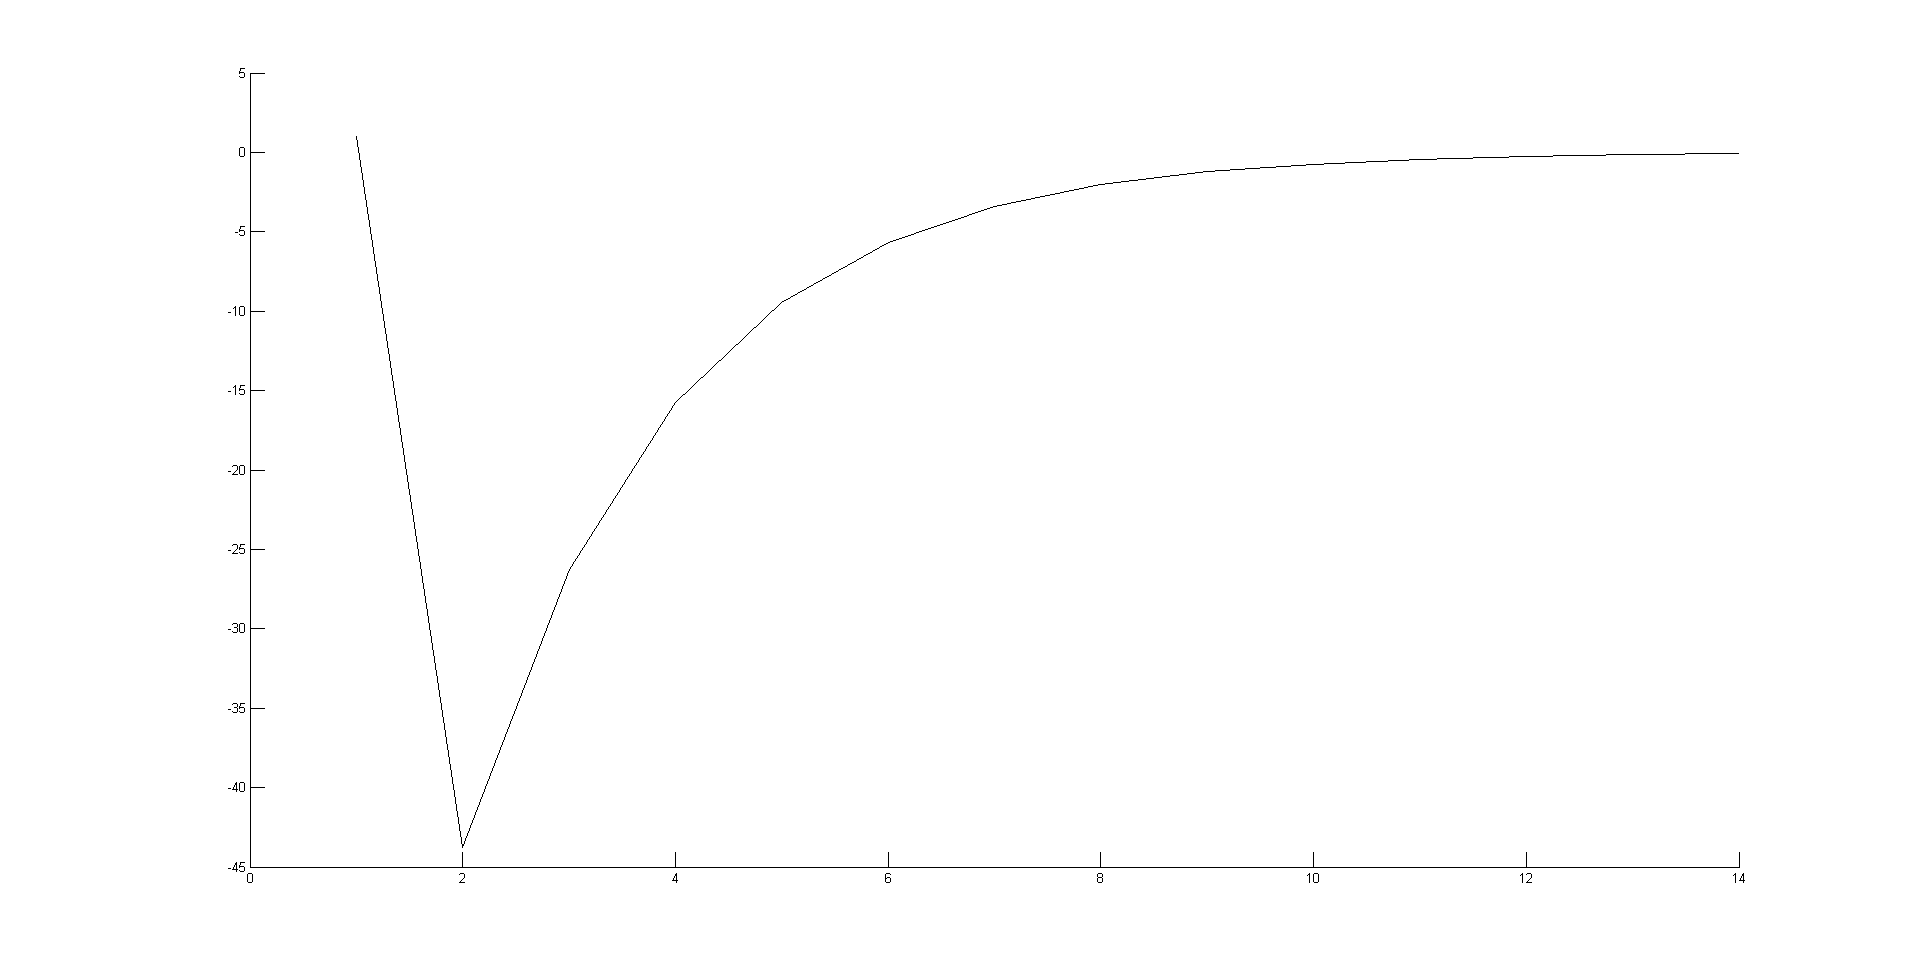
\includegraphics[width=120mm]{CW4-alg1fun1-u-24_5-k01-d.png}
	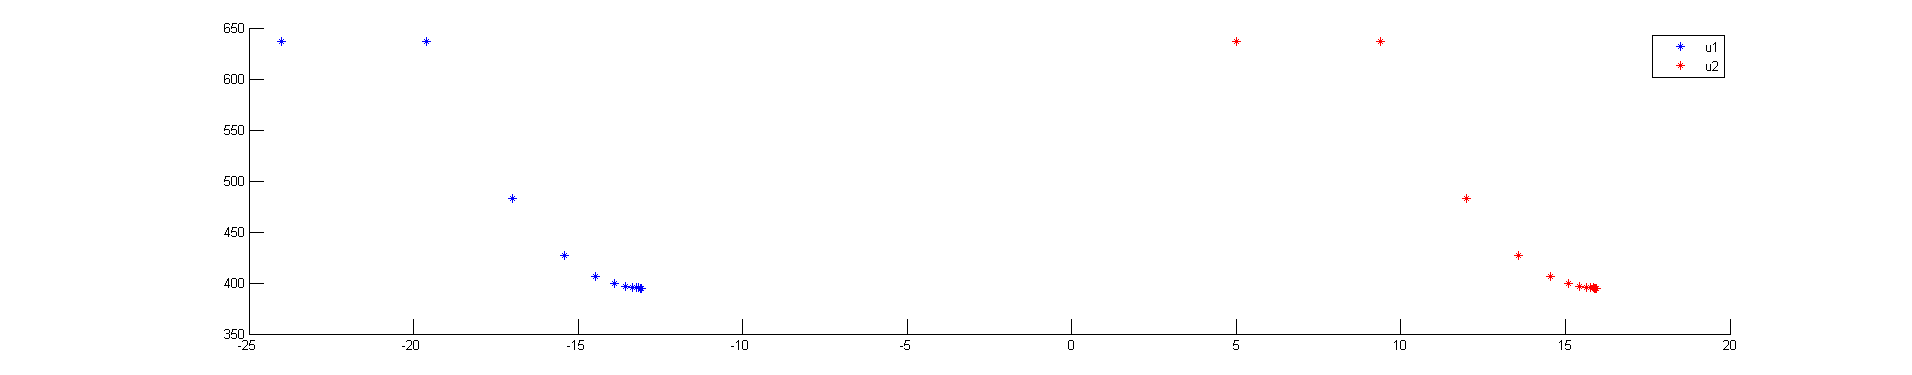
\includegraphics[width=120mm]{CW4-alg1fun1-u-24_5-k01-u.png}
	\caption{Wykres wykres wartości $d$, oraz $u^{(1)}$ i $u^{(2)}$ dla $u_0=[-24 \quad 5]$.}
    \label{fig:Rysunek}
\end{figure}

\newpage Z powyższych wykresów możemy zauważyć, że wartości $u^{(1)}$ i $u^{(2)}$ zmieniają się tak samo, a są jedynie przesunięte względem siebie o różnicę wartości początkowych $u_0^{(1)}$ i $u_0^{(2)}$, ponieważ w uproszczonym algorytmie nie mamy oddzielnych kroków $d^{(1)}$ i $d^{(2)}$ dla nich, ale jeden krok $d$ stosowany dla obu.

Następnie dla wybranych wartości początkowych wejścia $u_0$ ($[10 \quad 10]$) prześledzimy wpływ zmiany parametru $k$.
\begin{figure}[!h]
    \centering
	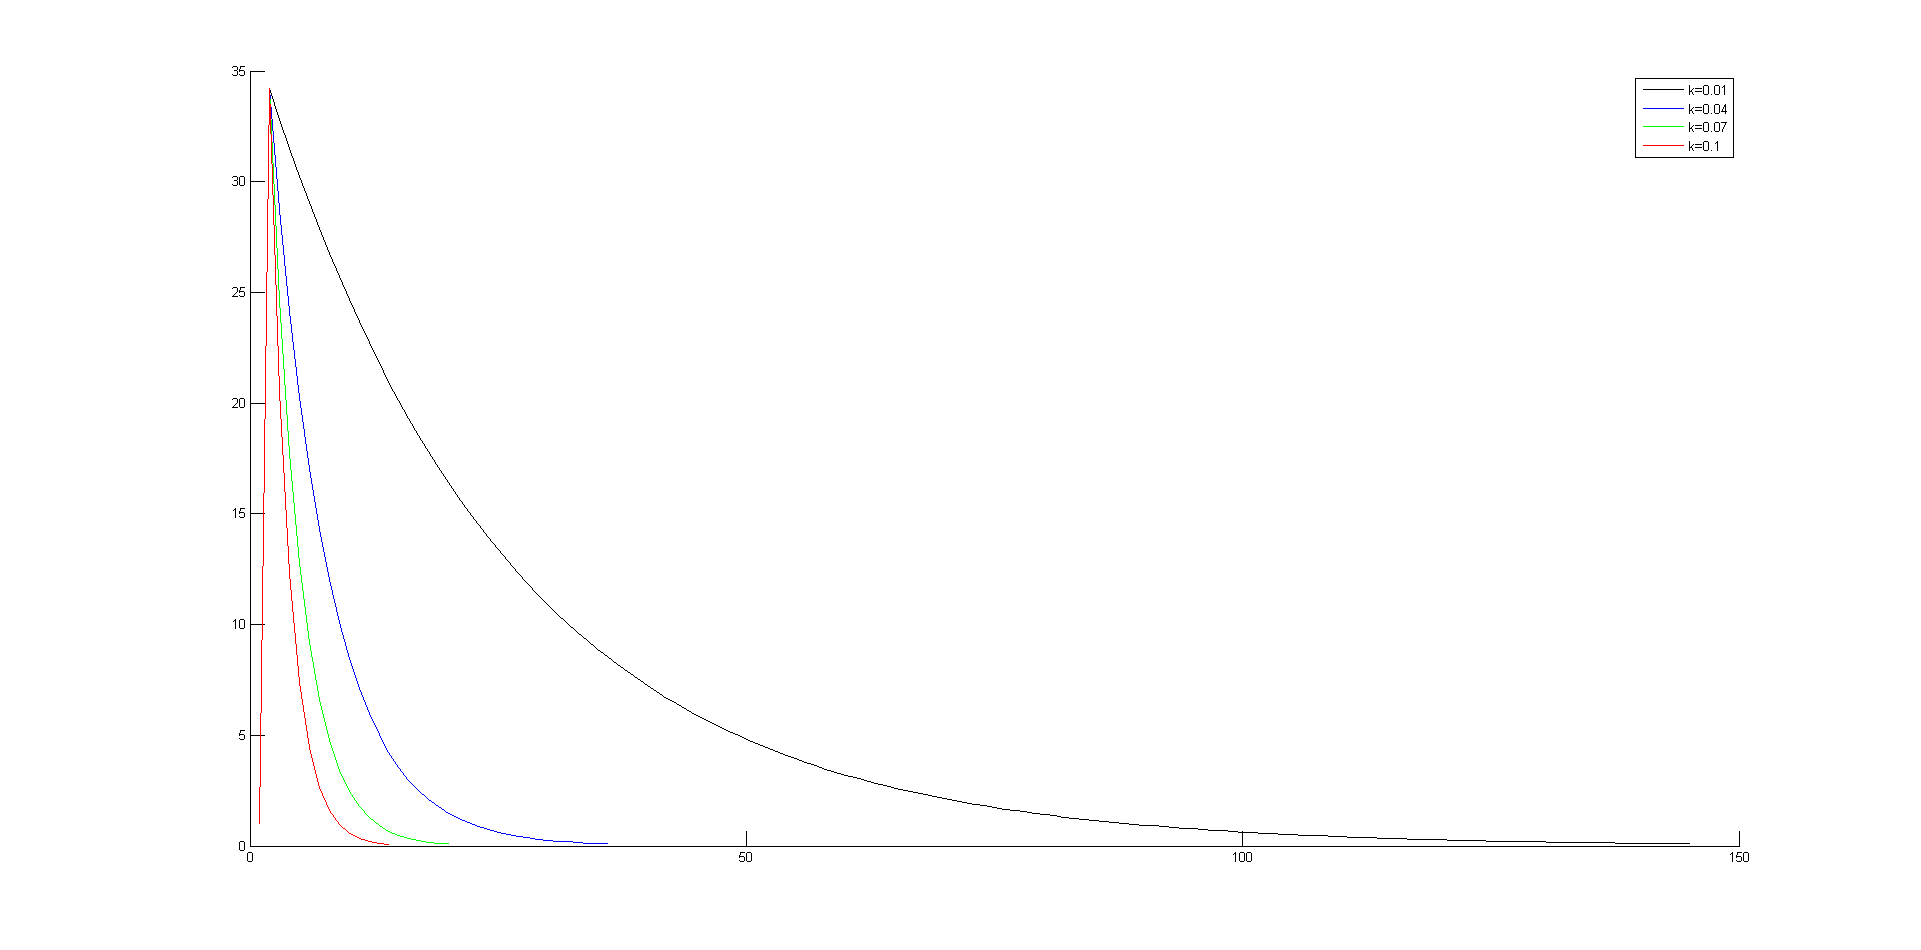
\includegraphics[width=120mm]{CW4-alg1fun1-u10_10-k001_01-d.png}
	\caption{Wykres wykres wartości $d$ przy zmianie parametru $k$.}
    \label{fig:Rysunek}
\end{figure}

Na powyższym wykresie możemy zauważyć, że w miarę zwiększania parametru $k$ wartości $d$ szybciej zbliżają się ku $0$.

\subsubsection{Obiekt (2).}

Wyjście drugiego obiektu w odróżnieniu od pierwszego zależy nie tylko od wejścia, ale i od czasu, więc przy sterowaniu nie wystarczy jednokrotne ustalenie wejść najlepszych do uzyskania ekstremum i należy powtarzać tę czynność co jakiś interwał czasowy. Jednak zauważyć możemy, że zmiany ekstremów w obiekcie 2 będą przebiegać okresowo, ponieważ w równaniu go opisującym czas jest argumentem funkcji sinus, dlatego też w tym ćwiczeniu rozpatrzymy przebieg sterowania dla trzech wartości parametru czasu $t$.

Testować będziemy wpływ parametru $k$, oraz stanu początkowego wejścia $u_0$ na przebieg sterowania przy użyciu odpowiedniej funkcji.
\begin{lstlisting}[caption=Funkcja testująca algorytm 1 dla obiektu 2.]
function alg1fun2(u, t, kstart, kstep, kstop)
    color = char('y', 'k', 'b', 'g', 'r', 'm');
    hold all;
    k = kstart;
    c = 1;
    
    while(k <= kstop)
        epsilon = 0.1;
        delta = 0.1
        u1(1) = u(1);
        u2(1) = u(2);
        y(1) = funkcja2([u(1) u(2)], t);
        i = 1;
        d(1) = 1;
        
        while(epsilon < abs(d(i)))
            a=(funkcja2([u1(i)+delta u2(i)+delta], t) - funkcja2([u1(i) u2(i)], t));
            d(i+1) =  a / delta;
            u1(i+1) = u1(i) - k * d(i+1);
            u2(i+1) = u2(i) - k * d(i+1);
            y(i+1)= funkcja2([u1(i) u2(i)], t);
            i = i + 1;
        end

        figure(1);
        hold on;
        plot(u1, y, '*b');
        plot(u2, y, '*r');
        figure(2);
        hold on;
        plot(d, strcat('-', color(mod(c,6)+1)));
       
        c = c + 1;
        k = k + kstep;
        clear u1; clear u2;  clear d; clear y;
    end
end
\end{lstlisting}

\begin{figure}[!h]
    \centering
	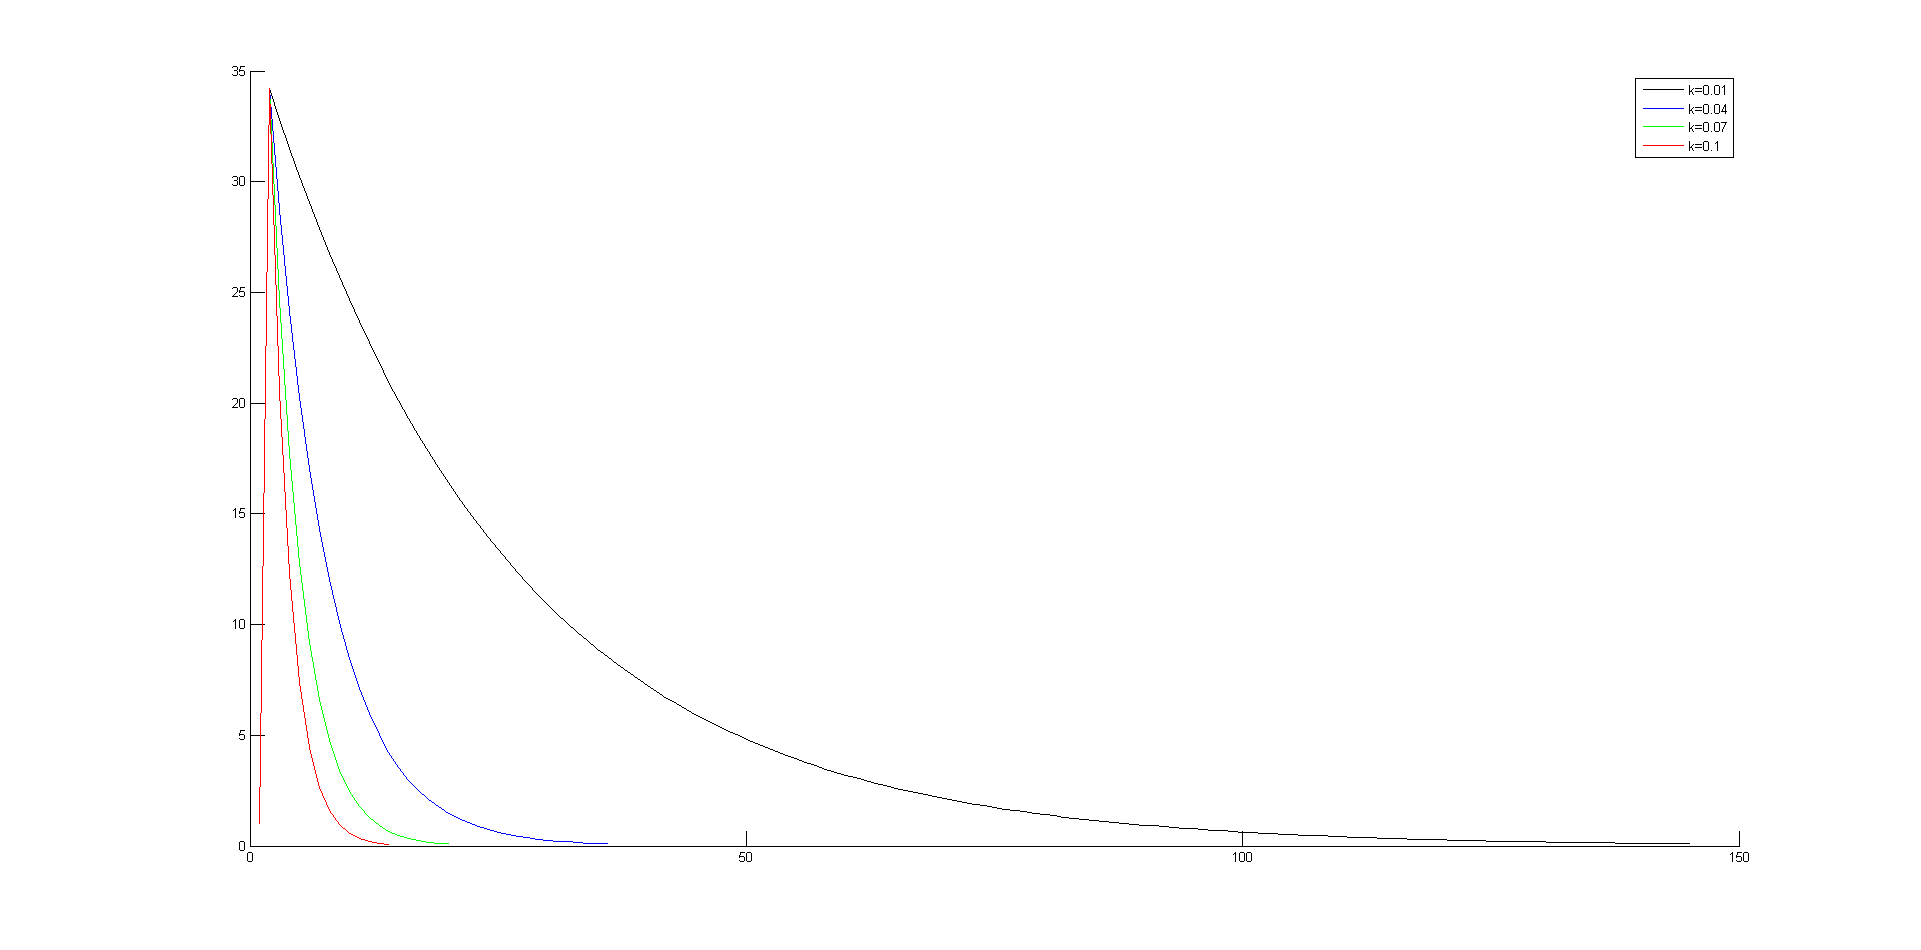
\includegraphics[width=120mm]{CW4-alg1fun2-u10_10-k001_01-t0-d.png}
	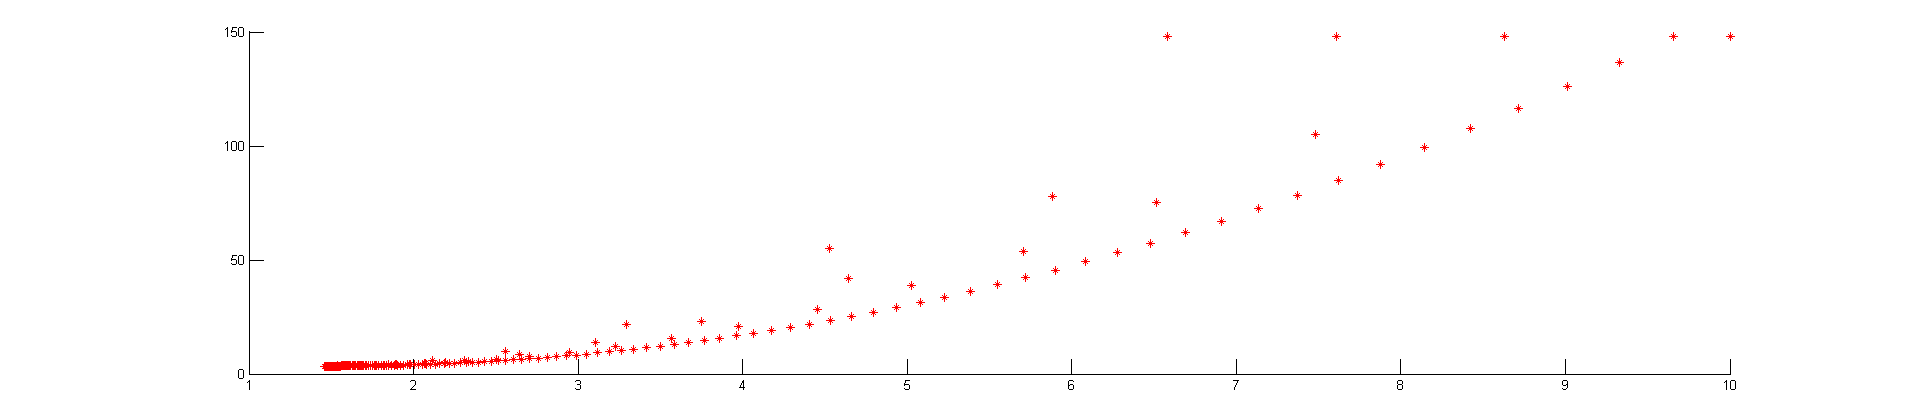
\includegraphics[width=120mm]{CW4-alg1fun2-u10_10-k001_01-t0-u.png}
	\caption{Wykres wykres wartości $d$, oraz $u^{(1)}$ i $u^{(2)}$ dla $u_0=[10 \quad 10]$ oraz $t=0$ przy zmieniającym się $k$.}
    \label{fig:Rysunek}
\end{figure}
\begin{figure}[!h]
    \centering
	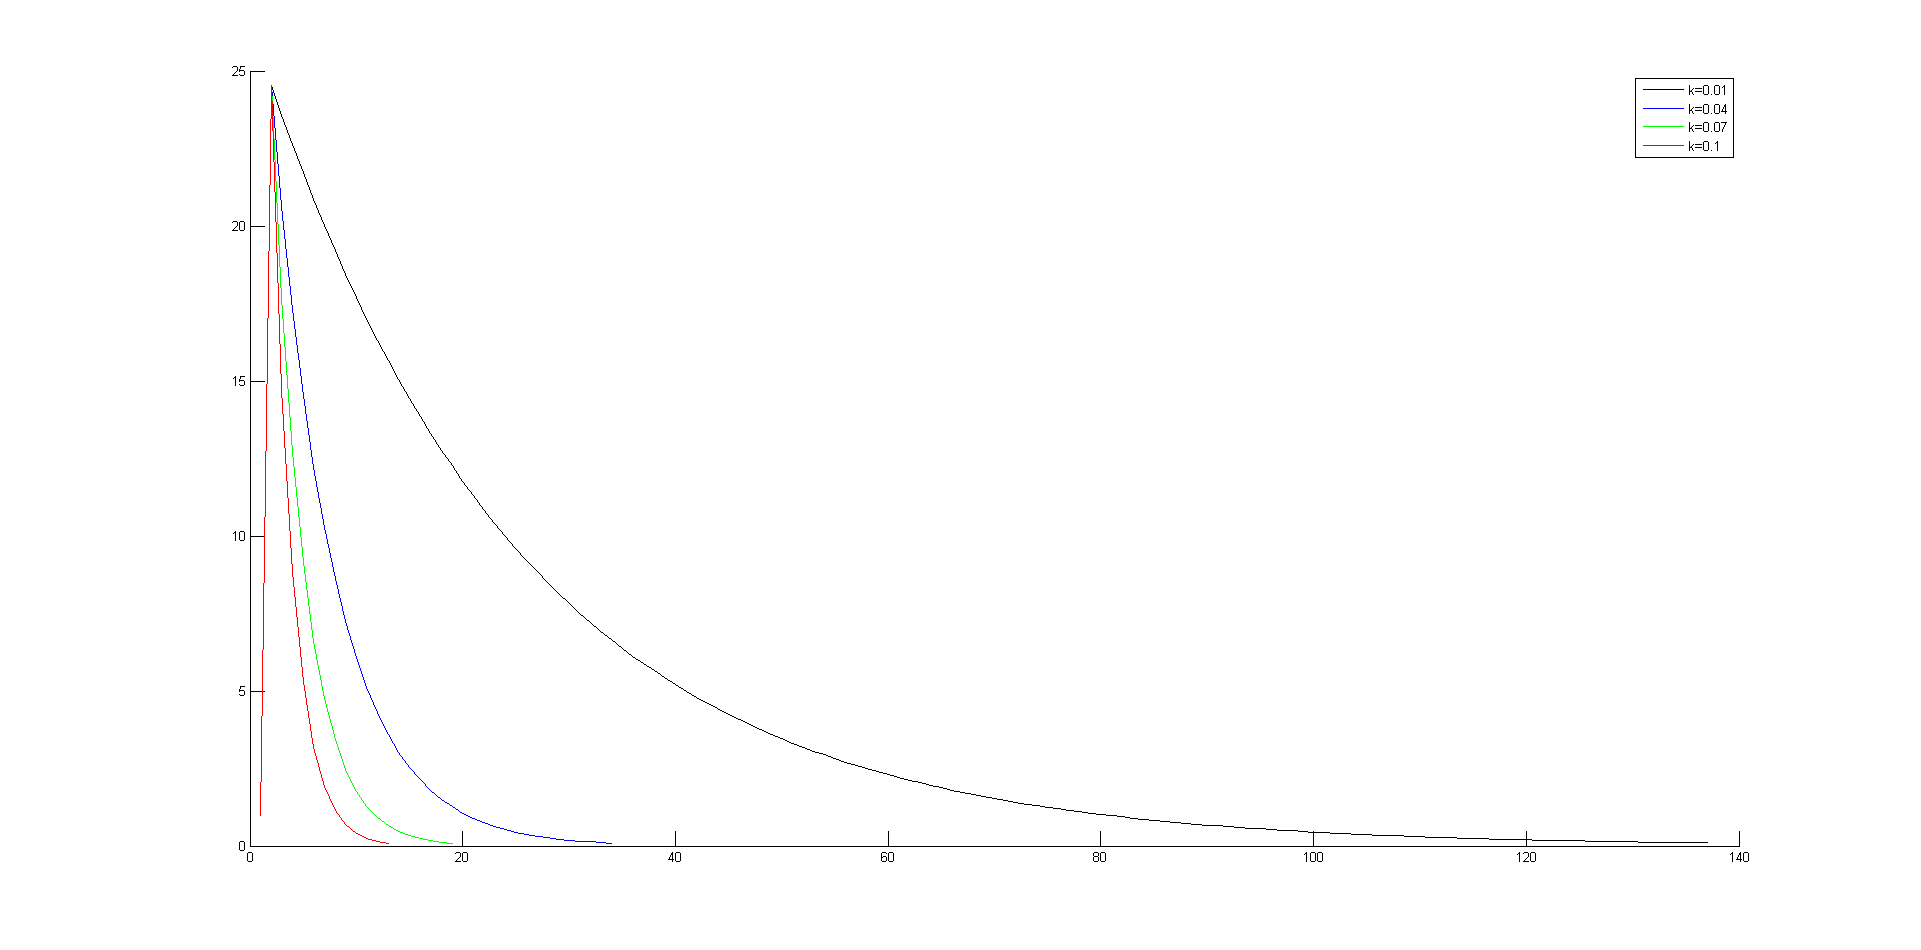
\includegraphics[width=120mm]{CW4-alg1fun2-u10_10-k001_01-t314-d.png}
	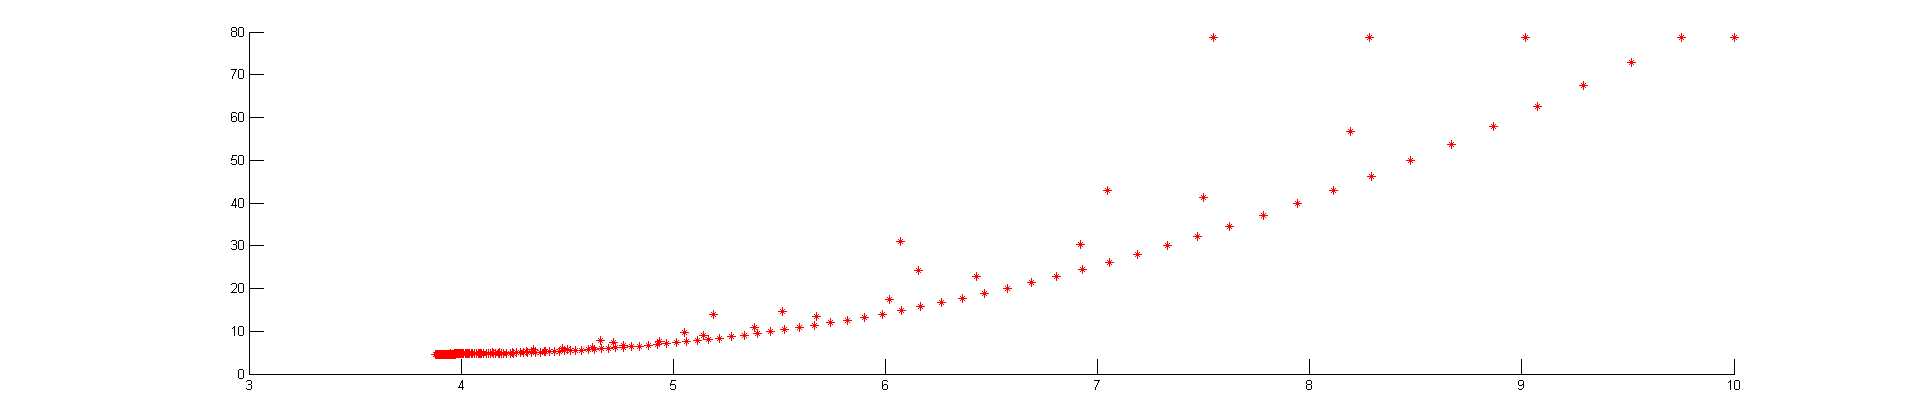
\includegraphics[width=120mm]{CW4-alg1fun2-u10_10-k001_01-t314-u.png}
	\caption{Wykres wykres wartości $d$, oraz $u^{(1)}$ i $u^{(2)}$ dla $u_0=[10 \quad 10]$ oraz $t=3.14$ przy zmieniającym się $k$.}
    \label{fig:Rysunek}
\end{figure}
\begin{figure}[!h]
    \centering
	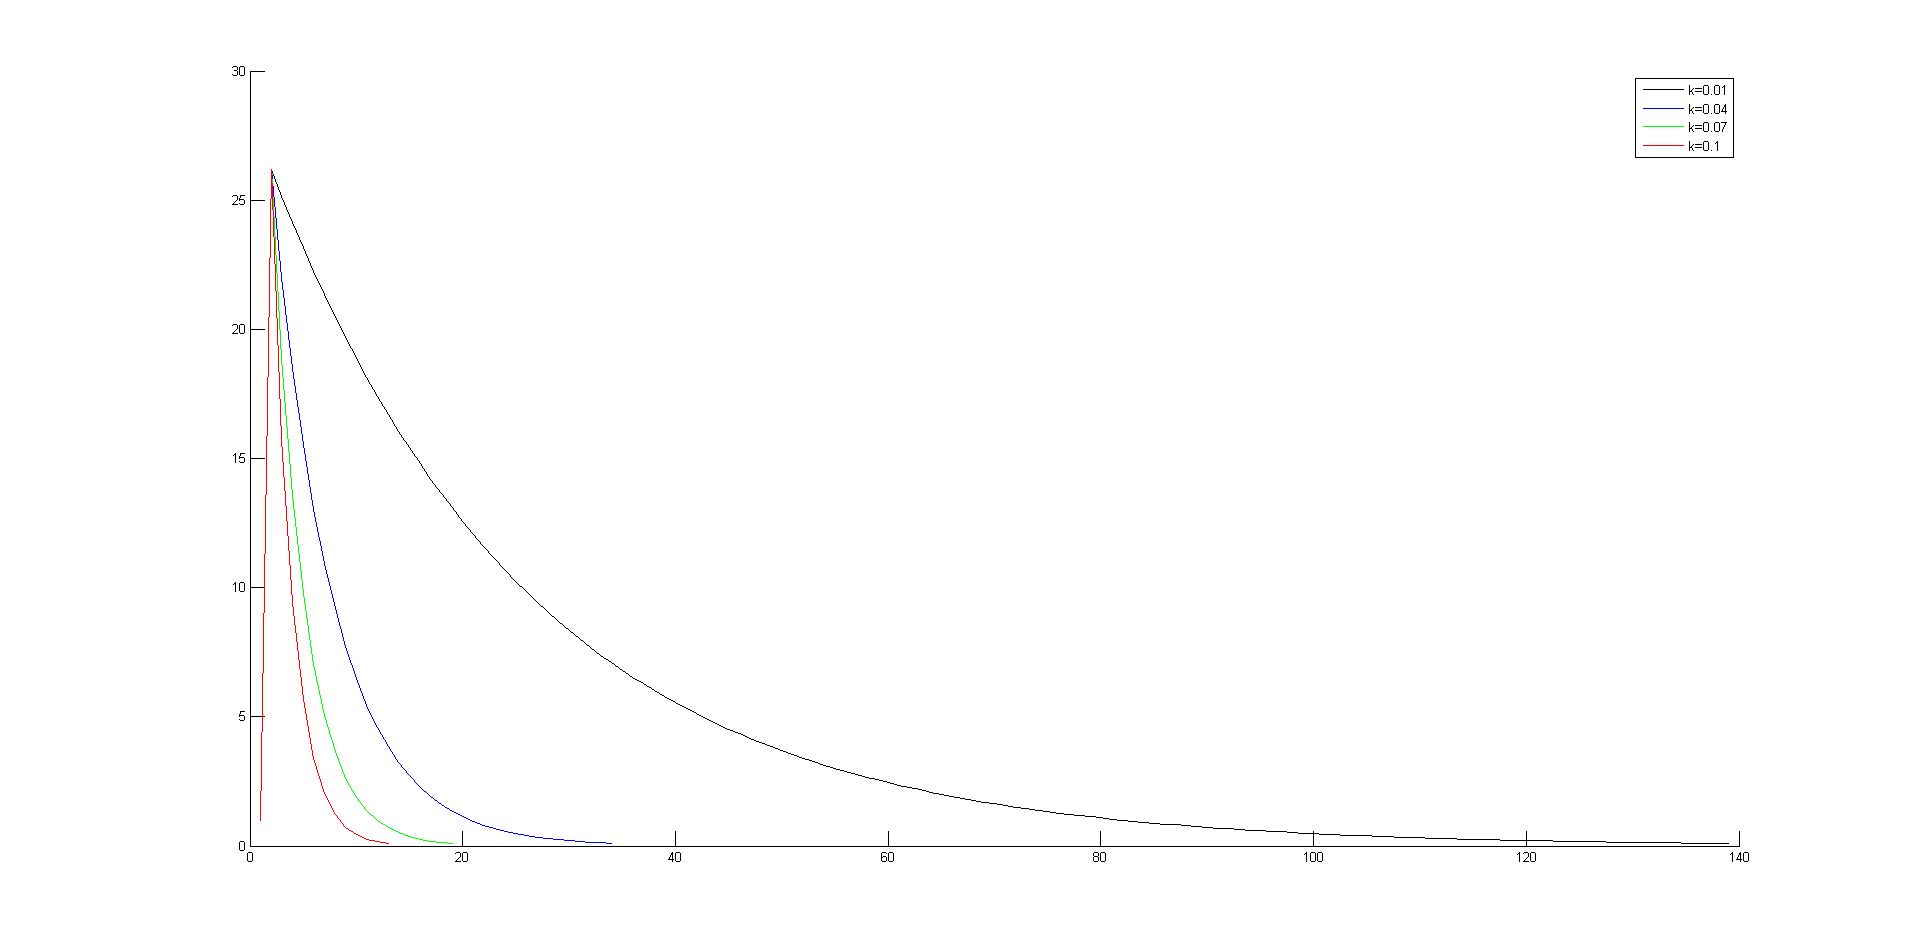
\includegraphics[width=120mm]{CW4-alg1fun2-u10_10-k001_01-t628-d.png}
	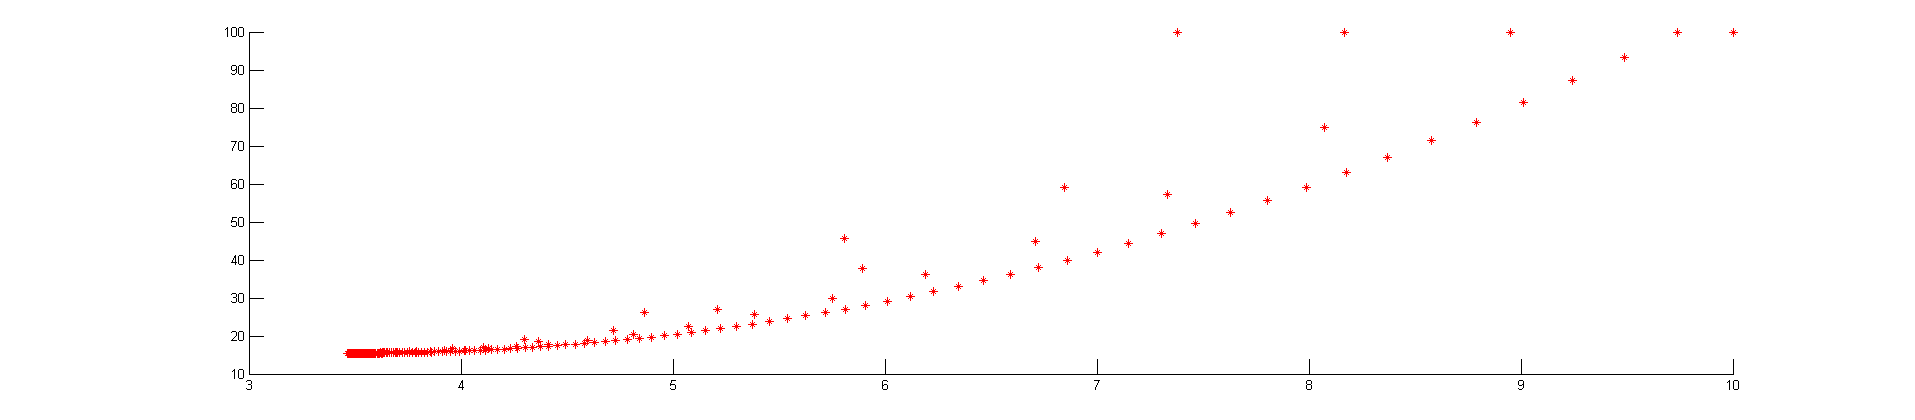
\includegraphics[width=120mm]{CW4-alg1fun2-u10_10-k001_01-t628-u.png}
	\caption{Wykres wykres wartości $d$, oraz $u^{(1)}$ i $u^{(2)}$ dla $u_0=[10 \quad 10]$ oraz $t=6.28$ przy zmieniającym się $k$.}
    \label{fig:Rysunek}
\end{figure}
\begin{figure}[!h]
    \centering
	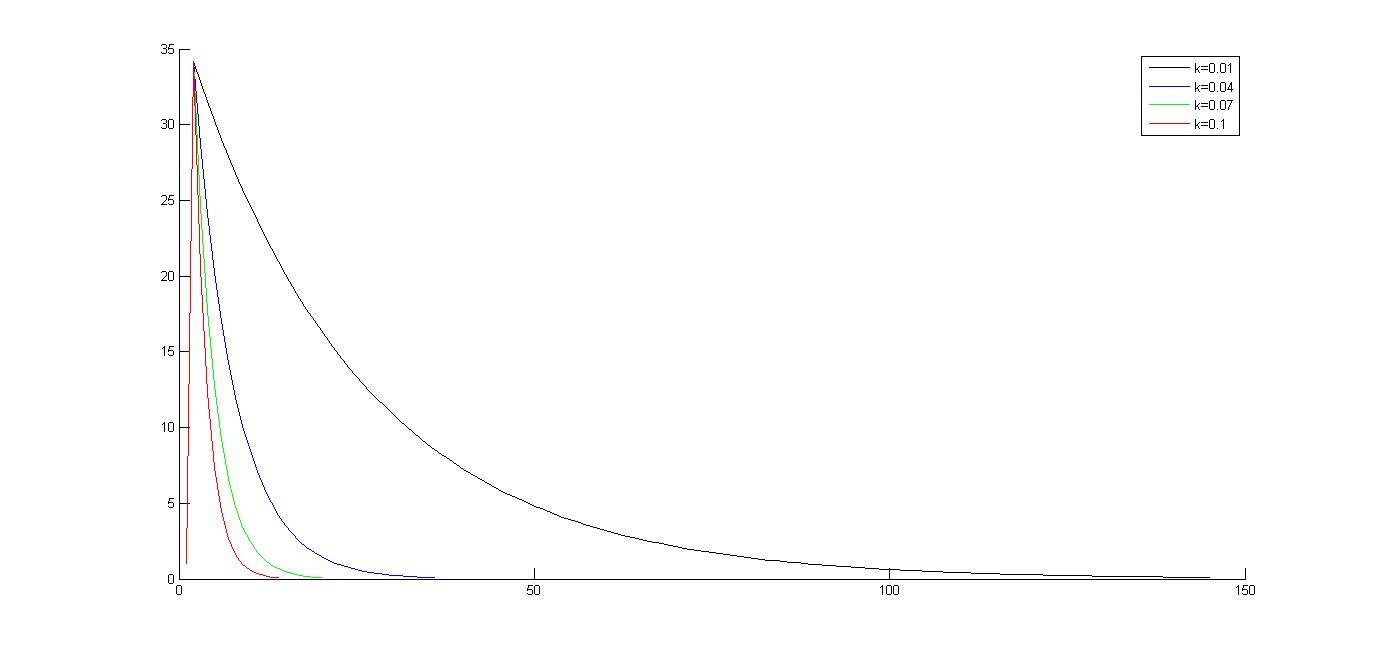
\includegraphics[width=120mm]{CW4-alg1fun2-u10_10-k001_01-t1256-d.png}
	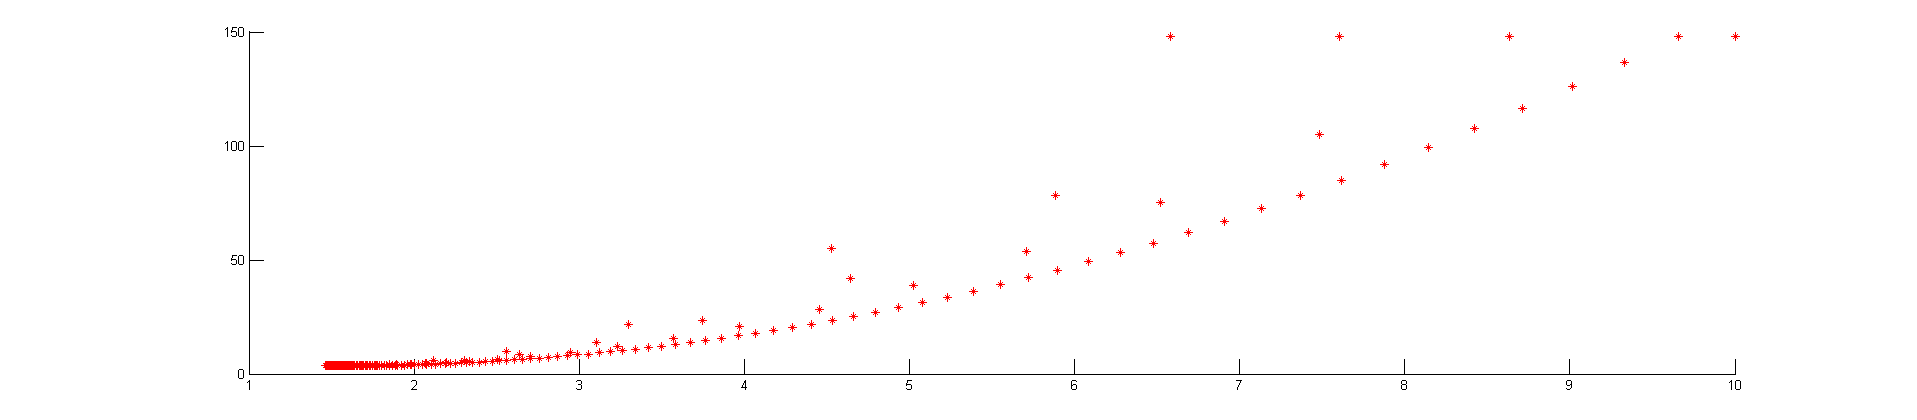
\includegraphics[width=120mm]{CW4-alg1fun2-u10_10-k001_01-t1256-u.png}
	\caption{Wykres wykres wartości $d$, oraz $u^{(1)}$ i $u^{(2)}$ dla $u_0=[10 \quad 10]$ oraz $t=12.56$ przy zmieniającym się $k$.}
    \label{fig:Rysunek}
\end{figure}

\newpage Z powyższych wykresów możemy zauważyć, że zmiana czasu nie wpływa na szybkość znalezienia ekstremum, oraz, że zawsze wraz ze wzrostem parametru $k$ liczba kroków potrzebna na zanalezienie ekstremum maleje. Zobaczyć możemy również, że dla różnych wartości czasu znalezione wartości $u$ różnią się, z wyjątkiem tych dla $t=0$, oraz $t=12.56 \approx 4\pi$, ponieważ różnica między nimi wynosi właśnie $4\pi$, czyli równa jest okresowi zmian ekstremów.

%--------------------------------------------------------------------------------------------------------------------------------
%ZADANIE 2
%--------------------------------------------------------------------------------------------------------------------------------
\subsection{Symulacja systemu sterowania ekstremalnego – wersja 2. algorytmu.}
\subsubsection{Obiekt (1).}
W drugim algorytmie znak kroku zależy od pochodnej przyrostowej.
\begin{eqnarray}
	u_n^{(i)} = u_{n-1}^{(i)}-kd_n^{(i)}\\
	d_n^{(i)} = sign \left[ {F(u_{n-1}) - F(u_{n-2}) \over u_{n-1}^{(i)} - u_{n-2}^{(i)}} \right] 
\end{eqnarray}
Uproszczenie:
\begin{eqnarray}
	u_n^{(i)} = u_{n-1}^{(i)}-kd_n\\
	d_n = sign \left[ {F([\begin{array}{ll} u_{n-1}^{(1)} + \Delta u & u_{n-1}^{(2)} + \Delta u\end{array}]) - F(u_{n-1}) \over \Delta u}\right] 
\end{eqnarray}
Do testowania algorytmu funkcja wyglada w następujący sposób:
\begin{lstlisting}[caption=Funkcja testująca algorytm 2 dla obiektu 1.]
function alg2fun1(u, kstart, kstep, kstop)
    color = char('y', 'k', 'b', 'g', 'r', 'm');
    hold all;
    k = kstart;
    c = 1;
    
    while(k <= kstop)
        epsilon = 0.1;
        delta = 0.1
        u1(1) = u(1);
        u2(1) = u(2);
        y(1) = funkcja1([u(1) u(2)]);
        i = 1;
        d(1) = 1;
        
        while(epsilon < abs(d(i)))
            a=(funkcja1([u1(i)+delta u2(i)+delta]) - funkcja1([u1(i) u2(i)]));
            d(i+1) =  a / delta;
            u1(i+1) = u1(i) - sign(a)*k * d(i+1);
            u2(i+1) = u2(i) - sign(a)*k * d(i+1);
            y(i+1)= funkcja1([u1(i) u2(i)]);
            i = i + 1;
        end
        figure(1);
        hold on;
        plot(u1, y, '*b');
        plot(u2, y, '*r');
        figure(2);
        hold on;
        plot(d, strcat('-', color(mod(c,6)+1)));
        c = c + 1;
        k = k + kstep;
        clear u1;
        clear u2;
        clear d;
        clear y;
    end
end
\end{lstlisting}


\newpage Dla stałego $k=0.1$ ustawiamy różne wartości $u_0$.
\begin{figure}[!h]
    \centering
	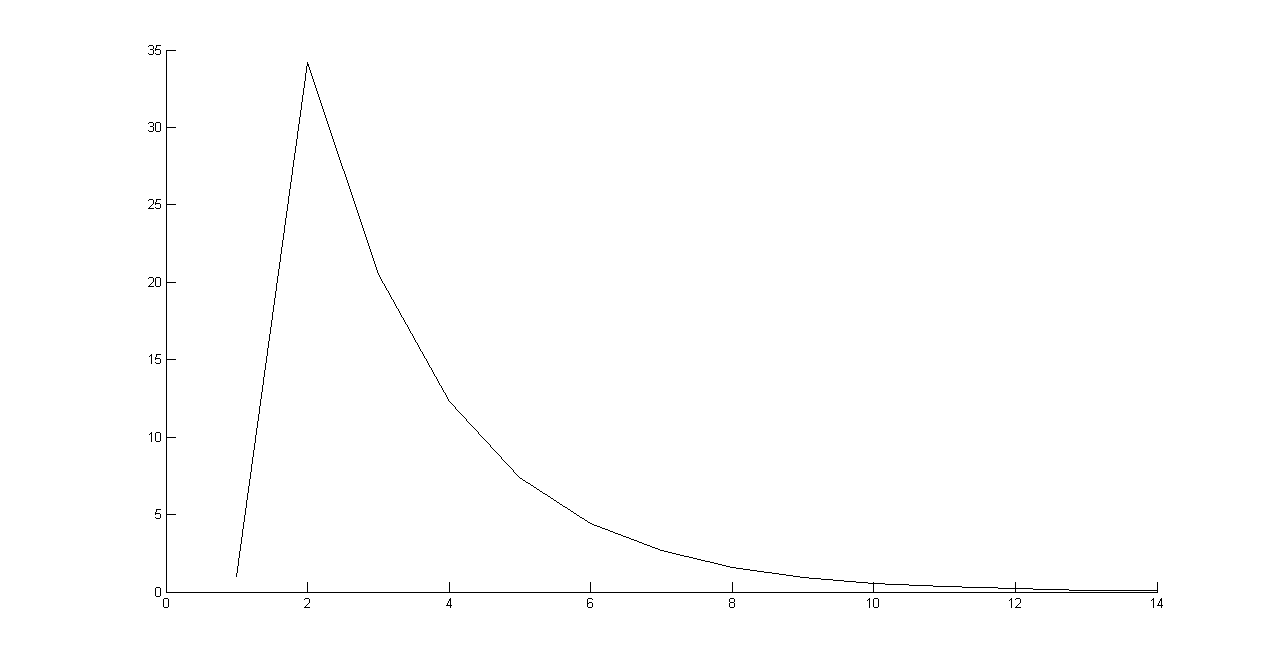
\includegraphics[width=120mm]{CW4-alg2fun1-u10_10-k01-d.png}
	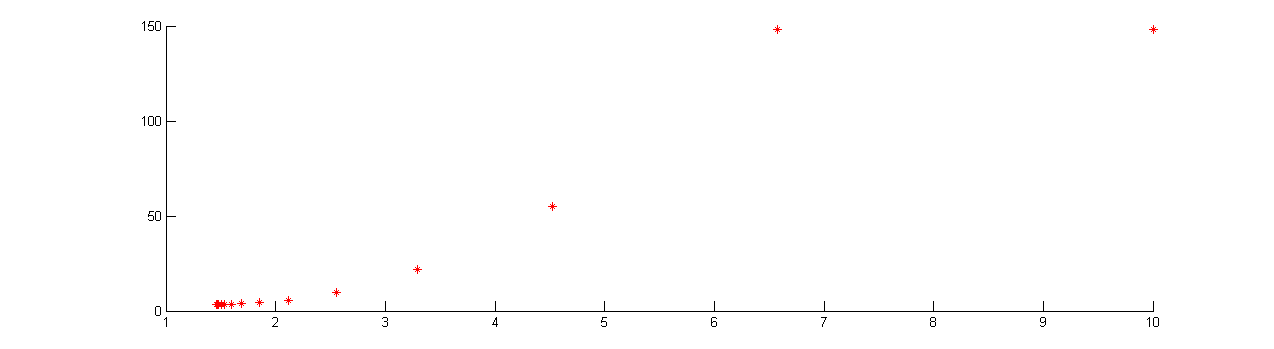
\includegraphics[width=120mm]{CW4-alg2fun1-u10_10-k01-u.png}
	\caption{Wykres wykres wartości $d$, oraz $u^{(1)}$ i $u^{(2)}$ dla $u_0=[10 \quad 10]$.\newline \small alg2fun1([10 10], 0.1, 0.1, 0.1) }
    \label{fig:Rysunek}
\end{figure}
\begin{figure}[!h]
    \centering
	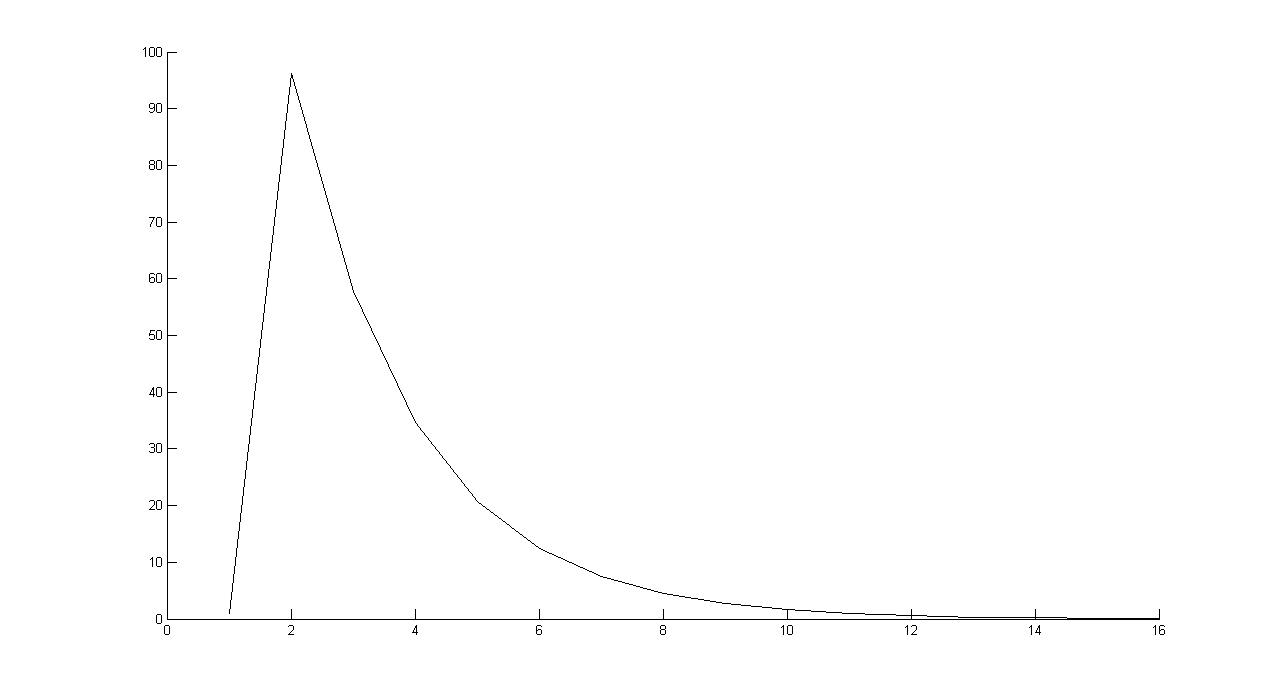
\includegraphics[width=120mm]{CW4-alg2fun1-u10_41-k01-d.png}
	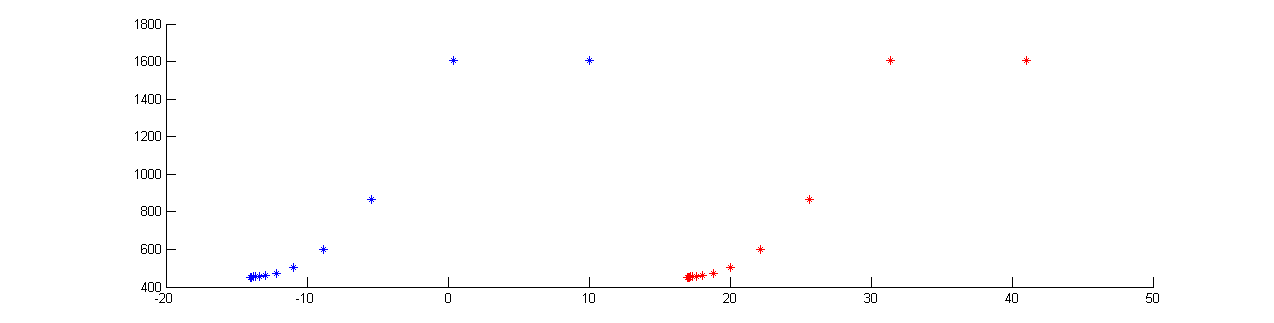
\includegraphics[width=120mm]{CW4-alg2fun1-u10_41-k01-u.png}
	\caption{Wykres wykres wartości $d$, oraz $u^{(1)}$ i $u^{(2)}$ dla $u_0=[10 \quad 41]$. \newline \small alg2fun1([10 41], 0.1, 0.1, 0.1)}
    \label{fig:Rysunek}
\end{figure}
\begin{figure}[!h]
    \centering
	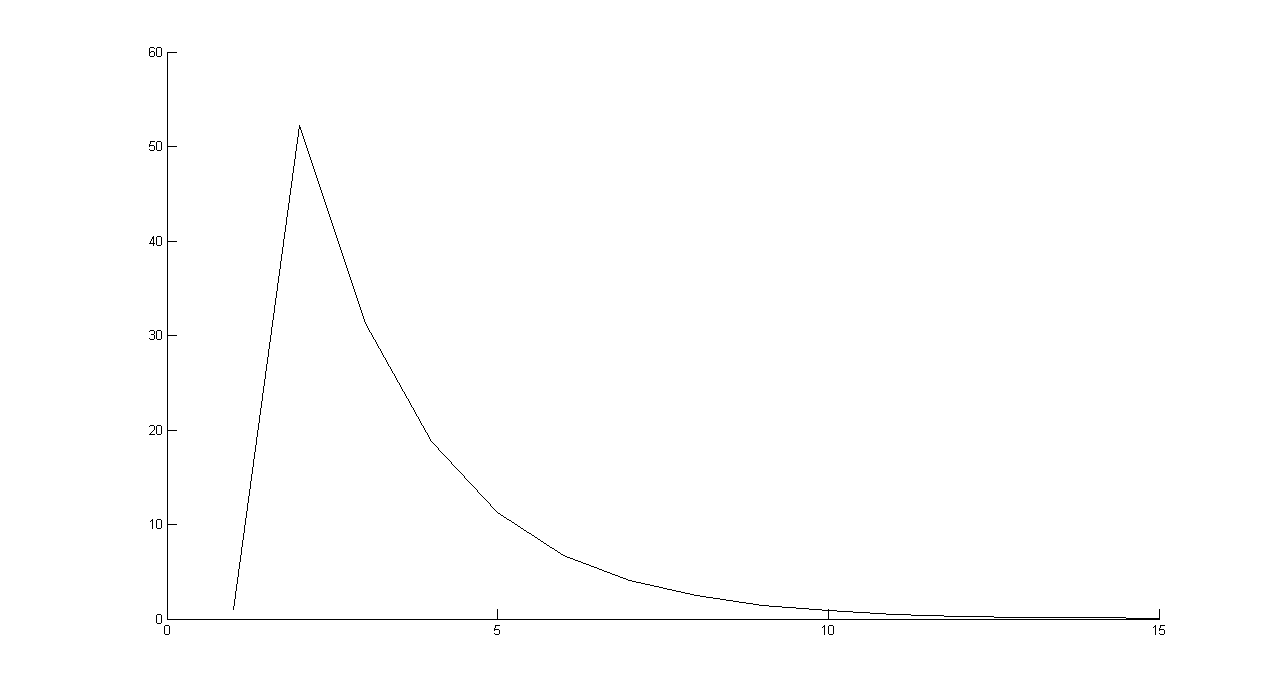
\includegraphics[width=120mm]{CW4-alg2fun1-u-24_5-k01-d.png}
	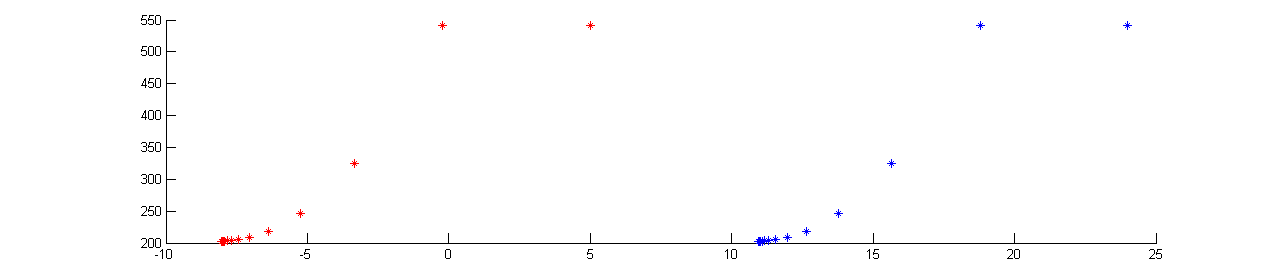
\includegraphics[width=120mm]{CW4-alg2fun1-u-24_5-k01-u.png}
	\caption{Wykres wykres wartości $d$, oraz $u^{(1)}$ i $u^{(2)}$ dla $u_0=[-24 \quad 5]$. \newline \small alg2fun1([24 5], 0.1, 0.1, 0.1)}
    \label{fig:Rysunek}
\end{figure}

Następnie zmieniane będzie $k$, a wartość stałą będzie miało  $u_0$ ($[10 \quad 10]$) $k$.

\begin{figure}[!h]
    \centering
	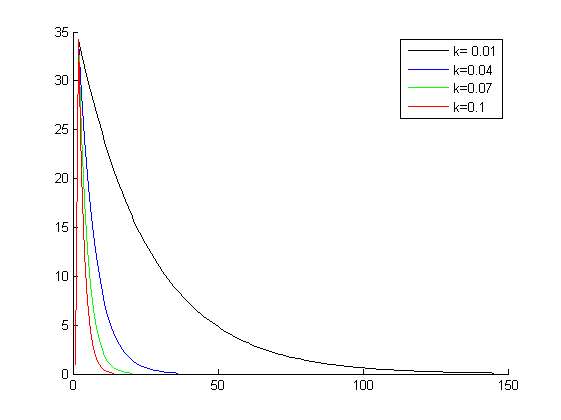
\includegraphics[width=120mm]{CW4-alg2fun1-u10_10-k001_01-d.png}
	\caption{Wykres wykres wartości $d$ przy zmianie parametru $k$. \newline \small alg2fun1([10 10], 0.01, 0.03, 0.1)}
    \label{fig:Rysunek}
\end{figure}


%TUUUUUUUUUU!!! PODSUMOWANIE

\subsubsection{Obiekt (2).}
%--------------------------------------------------------------------------------------------------------------------------------
%ZADANIE 3
%--------------------------------------------------------------------------------------------------------------------------------
\subsection{Symulacja systemu sterowania ekstremalnego – wersja 1. algorytmu.}

\subsubsection{Obiekt (1).}

\subsubsection{Obiekt (2).}
\section{Wnioski.}\label{sec:wnioski}

\end{document}